\section*{Respostas e Relatório de Ensaio}

\subsection*{Questão 4}
\begin{enumerate}
    \item[\textbf{a)}] $V = 1{,}644\text{ V}$
    
    \item[\textbf{b)}] $V = 1{,}353\text{ V}$. Observou-se uma redução na tensão de saída devido ao comportamento do sensor, cuja resistência elétrica diminui à medida que a temperatura aumenta.

\end{enumerate}



\subsection*{5. Cálculos de Tensão de Saída ($V_{out}$)}

\begin{equation*}
V_{out_1} = 5 \cdot \frac{8280}{20000} = 2,07\text{ V}
\end{equation*}

\begin{equation*}
V_{out_2} = 5 \cdot \frac{16,38 \cdot 10^3}{20000} = 4,095\text{ V}
\end{equation*}

\begin{equation*}
V_{out_3} = 5 \cdot \frac{21,51 \cdot 10^3}{20000} = 5,3775\text{ V}
\end{equation*}

\begin{equation*}
V_{out_4} = 5 \cdot \frac{23,85 \cdot 10^3}{20000} = 5,9625\text{ V}
\end{equation*}

\subsubsection*{2. Erro Relativo no Ponto Intermediário ($e_1$)}

\begin{align*}
V_{out, \text{medido}} &= 4,5\text{ V} \\
V_{out, \text{ideal}} &= 3,0\text{ V} \\[6pt]
e_1 &= 4,5 - 3,0 = 1,5\text{ V} \\[6pt]
\% e_1 &= \frac{e_1}{y_{\text{máx}} - y_{\text{mín}}} = \frac{1,5}{5 - 0} = 0,30
\end{align*}

\begin{align*}
y_{\text{máx}} &= 5\text{ V} \\
y_{\text{mín}} &= 0\text{ V}
\end{align*}

\subsubsection*{3. Erro Relativo no Ponto Final ($e_2$)}

\begin{align*}
V_{\text{out, calculado resistência medida}} &= 5,09624\text{ V} \\
V_{out, \text{ideal}} &= 5\text{ V} \\[6pt]
e_2 &= 5,09624 - 5 = 0,9624 \\[6pt]
\% e_2 &= \frac{0,9624}{5 - 0} = 0,1925
\end{align*}

\begin{figure}[h!] % [htbp] ajuda a posicionar a imagem no texto
    \centering
    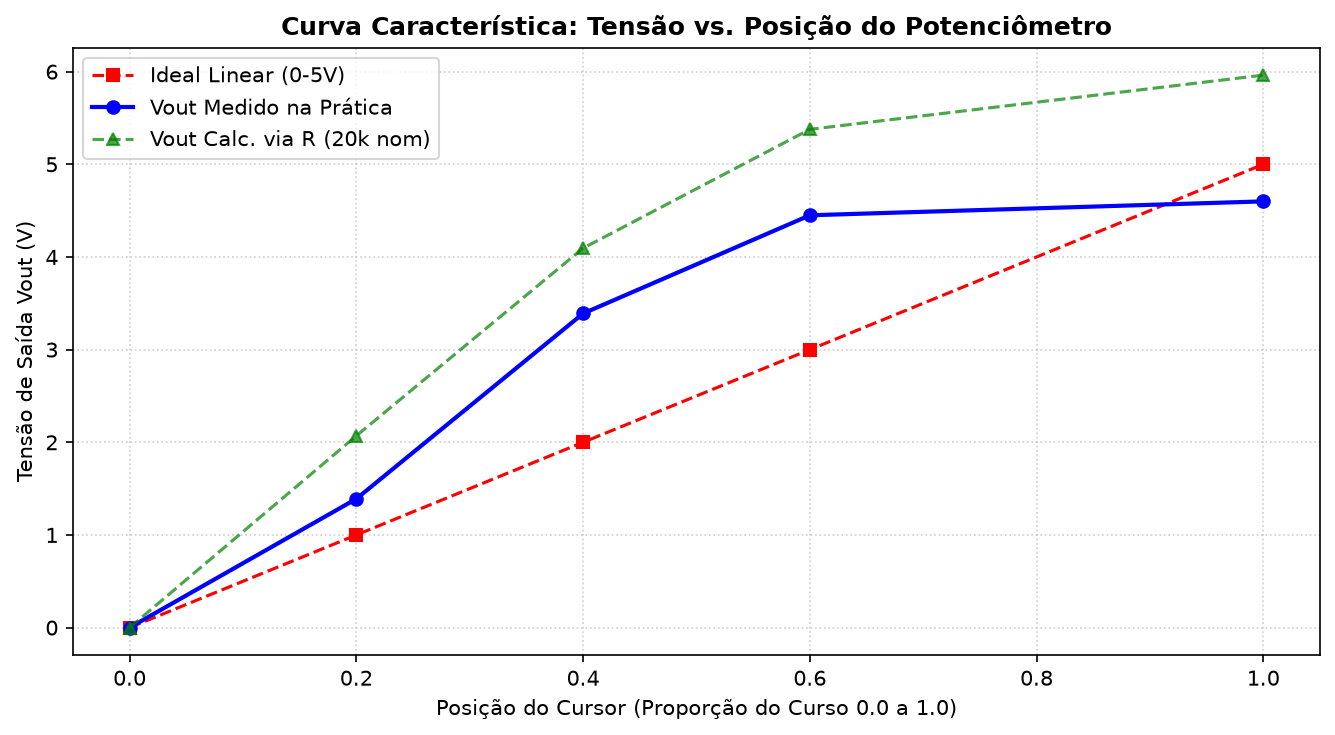
\includegraphics[width=0.7\linewidth]{curva.png} % Altere para o nome do seu arquivo
    \caption{plot das tensãoes medidas em laboratorio} % Legenda da imagem
    \label{fig:curva} % Rótulo para referenciar no texto
\end{figure}
\begin{table}[h!]
    \centering
    \caption{Valores teóricos, calculados e medidos da tensão de saída em função da posição.}
    \label{tab:resultados_completos}
    \begin{tabular}{c c c c c c}
        \toprule
        \textbf{Posição} & \textbf{R medida (k$\Omega$)} 
        & \textbf{$V_{out}$ teórico (V)}
        & \textbf{$V_{out}$ ($R_{nom}=20$ k$\Omega$)}
        & \textbf{$V_{out}$ ($R_{max}=23,65$ k$\Omega$)}
        & \textbf{$V_{out}$ medido (V)} \\
        \midrule
        0 cm & 0,00  & 0,00 & 0,00 & 0,00 & 0,00 \\
        1 cm & 8,28  & 1,00 & 2,07 & 1,75 & 1,39 \\
        2 cm & 16,38 & 2,00 & 4,10 & 3,46 & 3,39 \\
        3 cm & 21,51 & 3,00 & 5,38 & 4,55 & 4,45 \\
        5 cm & 23,65 & 5,00 & 5,91 & 5,00 & 4,60 \\
        \bottomrule
    \end{tabular}
\end{table}
Como pode ser observado na Figura \ref{fig:curva}, a curva da tensão de saída em função da resistência medida apresenta uma diferença em relação aos valores obtidos experimentalmente. Nos cálculos realizados considerando \(R_{nom}=20\,\mathrm{k}\Omega\), a tensão de saída atinge valores superiores a \(5\,\mathrm{V}\), chegando aproximadamente a \(5,91\,\mathrm{V}\). Esse comportamento ocorre devido à utilização de um modelo matemático idealizado, no qual a tensão de saída é determinada diretamente pela razão entre a resistência medida e a resistência nominal do potenciômetro. Dessa forma, como a resistência medida em algumas posições ultrapassa o valor nominal de \(20\,\mathrm{k}\Omega\), o cálculo resulta em uma tensão superior à tensão de referência de \(5\,\mathrm{V}\).

Entretanto, fisicamente, o circuito está limitado pela tensão de alimentação de aproximadamente \(5\,\mathrm{V}\), de modo que a tensão de saída não pode simplesmente assumir valores superiores a essa alimentação. Além disso, as tolerâncias dos componentes, a resistência efetiva do potenciômetro e as características do circuito de medição contribuem para a diferença entre os valores teóricos e experimentais. Isso explica por que, apesar de o modelo calculado apresentar valores de até \(5,91\,\mathrm{V}\), a maior tensão observada experimentalmente foi de aproximadamente \(4,60\,\mathrm{V}\).



\subsection*{Questão 6}
\begin{enumerate}
    \item[\textbf{a)}] Ao aproximar o primeiro polo do ímã, não foi observada nenhuma alteração no estado do circuito (o LED permaneceu inalterado).
    
    \item[\textbf{b)}] Ao aproximar o polo oposto do ímã, o LED apagou.
    
    \item[\textbf{c)}] O LED acende na primeira aproximação e não apaga na segunda aproximação.
    
    \item[\textbf{d)}] O componente é um \textbf{Sensor de Efeito Hall do tipo Bipolar}. Seu funcionamento é caracterizado pela retenção de estado (efeito \textit{latch}): a saída é ativada (apagando o LED) pela presença de um polo \textbf{Sul} (campo magnético positivo) e desativada pela presença de um polo \textbf{Norte} (campo magnético negativo).

\end{enumerate}

\end{document}